
% DARPA CASE
Developers of safety-critical embedded systems have become increasingly aware that their products are vulnerable and subject to cyber attacks similar to those common in large enterprise networks.  In response, efforts are underway to incorporate \textit{cyber-resiliency} into system design.  Cyber-resiliency means that the system is tolerant to cyber attacks just as safety-critical systems are tolerant to random faults: they recover and continue to execute their mission function, or safely shut down, as requirements dictate.  Unfortunately, systems engineers are currently given few development tools to help answer even basic questions about potential vulnerabilities and mitigations, and instead rely on process-oriented checklists and guidelines.

The DARPA Cyber Assured Systems Engineering (CASE) program was launched to research new methods and tools for design, analysis, and verification that enable systems engineers to \textit{design-in} cyber-resiliency for complex cyber-physical systems. 
%
% BRIEFCASE TOOLS AND FEATURES
Our team developed BriefCASE~\cite{case-at-scale}, a framework for developing and assuring cyber-resilient embedded systems according to the CASE workflow depicted in Fig.~\ref{fig:workflow}. BriefCASE provides a development environment for modeling system architectures in AADL~\cite{feiler-aadl}, analyzing the models for cyber-vulnerabilities, mitigating those vulnerabilities by applying automated model transformations, formally verifying security properties in the model, generating high-assurance component code from model specifications, building the system to a secure kernel target, and finally, generating a system cyber-resiliency assurance case.  

\begin{figure}[h] 
	\centering 
	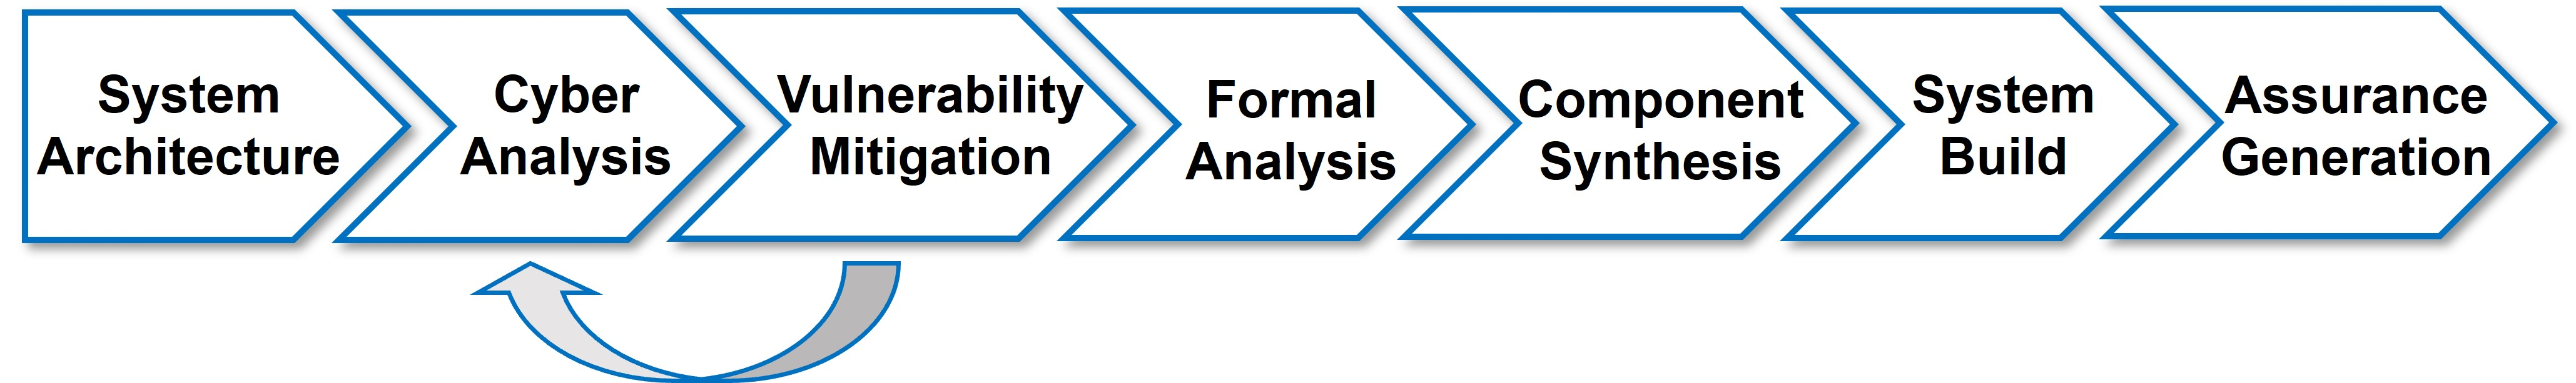
\includegraphics[width=\columnwidth]{figs/workflow.jpg}
	\caption{Cyber Assured Systems Engineering workflow.}
	\label{fig:workflow} 
\end{figure}

% ASSURANCE
For the development of high-assurance systems, multiple stakeholders must be convinced of the system's dependability prior to deployment.  First and foremost, the developer must be confident that the system operates correctly with respect to the intent of the specification.  Next, the certification or accreditation authority (where applicable) must be convinced.  Finally the customer, end user (and often other stakeholders in between) will need \textit{assurance} that the system will behave as intended.  
Assurance is defined as the ``planned and systematic actions necessary to provide adequate confidence and evidence that a product or process satisfies given requirements"~\cite{do-178c}, and different stakeholders may require different means of assurance.  

A structured \textit{assurance argument} is one method for conveying assurance.
In order to be effective, the argument should be well-formed, complete, and substantiated with evidence.    
Arguments can be constructed manually or based on assurance \textit{patterns}, in which generic arguments are defined (ideally arrived at through consensus by a body of experts), then instantiated with a concrete system instance~\cite{Kelly97:patterns}.  This is the approach taken by BriefCASE, which includes a collection of \textit{hierarchical} cybersecurity assurance patterns that are instantiated with the system under development and incorporate evidence from artifacts generated by the framework.  
%The assurance patterns are hierarchical in that they are represented as \textit{modules} that can be composed into a comprehensive pattern for addressing specific dependability concerns.
The assurance patterns are hierarchical in that the argument embodied in one pattern may be used to help substantiate the claim made by another pattern.  The patterns are  represented as \textit{modules} that can be composed into larger, comprehensive patterns for addressing specific dependability concerns. 
%
Patterns for assurance case argumentation have been considered in~\cite{Denney13:pattern}, \cite{Hawkins11:pattern}, \cite{Kelly97:patterns}, and~\cite{Sun11:pattern}. An approach to apply and evolve assurance cases as part of system design is found in~\cite{Graydon07:dev}, which is similar to the process we use in BriefCASE.

In previous work~\cite{resolute-destion}, we described assurance patterns corresponding to specific BriefCASE cyber-vulnerability mitigations.  However, we only provided a high-level summary of those patterns, and they primarily focused on assuring that security requirements were satisfied in the design by examining the model structure (for example, demonstrating that an inserted filter component could not be bypassed).
%%However, those patterns primarily focused on assuring that aspects of security requirements were satisfied in the design by examining the model structure (for example, demonstrating that an inserted filter component could not be bypassed).  
%%Moreover,~\cite{resolute-destion} is a short-format paper that only gives a very high-level summary of the selected patterns.
%%
%% CONTRIBUTION AND PAPER OUTLINE
In this paper we significantly expand on that work by presenting a more comprehensive collection of hierarchical CASE assurance patterns covering the generation and ingestion of cyber requirements, requirement satisfaction in the model, and requirement satisfaction in the realization of the model.  In addition, we describe the mechanisms by which evidence generated as part of the BriefCASE workflow is incorporated into an instantiated assurance case.
%
%The high-level structure of our CASE assurance patterns is inspired in part by the D-MILS argument pattern~\cite{dmils}, in which system dependability properties are assured via modules arguing component, compositional, and implementation correctness.  Similar to BriefCASE, the authors demonstrate how to instantiate the D-MILS pattern from an AADL system model; however, they accomplish this via specification of an additional \textit{weaving model}, which is not necessary in BriefCASE due to the tight coupling between the modeling environment and assurance tool.
%
%The VERDICT~\cite{verdict} framework was also developed on the CASE program and has some similarities with BriefCASE.  Although VERDICT does generate and evaluate assurance arguments based on analyses performed as part of the tool workflow, the assurance arguments are only shallow fragments of a comprehensive cybersecurity case, and focus primarily on whether applicable Common Attack Pattern Enumerations and Classifications (CAPEC)~\cite{capec} have been addressed in the design.  In contrast, our CASE assurance patterns consider vulnerability mitigations in the system design \textit{and} the implementation, and include arguments for several other aspects of cyber-resiliency assurance as well.
%
%
%AMASS~\cite{AMASS} is another framework that incorporates a workflow similar to BriefCASE.  \todo{Finish this description}
%
%\todo{Describe other cybersecurity assurance patterns (NIST, etc)}

The remainder of this paper is organized as follows. In Section~\ref{sec:related-work}, we describe related research on cybersecurity assurance patterns and frameworks. In Section~\ref{sec:briefcase}, we present an overview of the BriefCASE framework and workflow. Section~\ref{sec:assurance-pattern} describes our assurance patterns with respect to that workflow. Specifically, we focus on arguments for security requirement correctness, model correctness, and implementation correctness.  We provide concluding remarks and discuss future directions in Section~\ref{sec:conclusion}.